%!TeX root=../wowtop.tex

\ArtChapter[Wreckage]{26head}

\lettrine[lines=4,findent=2pt]{A}{nd} now comes the strangest thing in my story. Yet, perhaps, it is not altogether strange. I remember, clearly and coldly and vividly, all that I did that day until the time that I stood weeping and praising God upon the summit of Primrose Hill. And then I forget.

Of the next three days I know nothing. I have learned since that, so far from my being the first discoverer of the Martian overthrow, several such wanderers as myself had already discovered this on the previous night. One man—the first—had gone to St~Martin's-le-Grand, and, while I sheltered in the cabmen's hut, had contrived to telegraph to Paris. Thence the joyful news had flashed all over the world; a thousand cities, chilled by ghastly apprehensions, suddenly flashed into frantic illuminations; they knew of it in Dublin, Edinburgh, Manchester, Birmingham, at the time when I stood upon the verge of the pit. Already men, weeping with joy, as I have heard, shouting and staying their work to shake hands and shout, were making up trains, even as near as Crewe, to descend upon London. The church bells that had ceased a fortnight since suddenly caught the news, until all England was bell-ringing. Men on cycles, lean-faced, unkempt, scorched along every country lane shouting of unhoped deliverance, shouting to gaunt, staring figures of despair. And for the food! Across the Channel, across the Irish Sea, across the Atlantic, corn, bread, and meat were tearing to our relief. All the shipping in the world seemed going Londonward in those days. But of all this I have no memory. I drifted—a demented man. I found myself in a house of kindly people, who had found me on the third day wandering, weeping, and raving through the streets of St~John's Wood. They have told me since that I was singing some insane doggerel about »The Last Man Left Alive! Hurrah! The Last Man Left Alive!« Troubled as they were with their own affairs, these people, whose name, much as I would like to express my gratitude to them, I may not even give here, nevertheless cumbered themselves with me, sheltered me, and protected me from myself. Apparently they had learned something of my story from me during the days of my lapse.

\begin{figure}[tb]
\centering

\includegraphics[width=\linewidth]{26workmen}
%\caption{Harmless in the brightness of the rising sun}
\end{figure}

Very gently, when my mind was assured again, did they break to me what they had learned of the fate of Leatherhead. Two days after I was imprisoned it had been destroyed, with every soul in it, by a Martian. He had swept it out of existence, as it seemed, without any provocation, as a boy might crush an ant hill, in the mere wantonness of power.

I was a lonely man, and they were very kind to me. I was a lonely man and a sad one, and they bore with me. I remained with them four days after my recovery. All that time I felt a vague, a growing craving to look once more on whatever remained of the little life that seemed so happy and bright in my past. It was a mere hopeless desire to feast upon my misery. They dissuaded me. They did all they could to divert me from this morbidity. But at last I could resist the impulse no longer, and, promising faithfully to return to them, and parting, as I will confess, from these four-day friends with tears, I went out again into the streets that had lately been so dark and strange and empty.

Already they were busy with returning people; in places even there were shops open, and I saw a drinking fountain running water.

I remember how mockingly bright the day seemed as I went back on my melancholy pilgrimage to the little house at Woking, how busy the streets and vivid the moving life about me. So many people were abroad everywhere, busied in a thousand activities, that it seemed incredible that any great proportion of the population could have been slain. But then I noticed how yellow were the skins of the people I met, how shaggy the hair of the men, how large and bright their eyes, and that every other man still wore his dirty rags. Their faces seemed all with one of two expressions—a leaping exultation and energy or a grim resolution. Save for the expression of the faces, London seemed a city of tramps. The vestries were indiscriminately distributing bread sent us by the French government. The ribs of the few horses showed dismally. Haggard special constables with white badges stood at the corners of every street. I saw little of the mischief wrought by the Martians until I reached Wellington Street, and there I saw the red weed clambering over the buttresses of Waterloo Bridge.

At the corner of the bridge, too, I saw one of the common contrasts of that grotesque time—a sheet of paper flaunting against a thicket of the red weed, transfixed by a stick that kept it in place. It was the placard of the first newspaper to resume publication—the \textit{Daily Mail}. I bought a copy for a blackened shilling I found in my pocket. Most of it was in blank, but the solitary compositor who did the thing had amused himself by making a grotesque scheme of advertisement stereo on the back page. The matter he printed was emotional; the news organisation had not as yet found its way back. I learned nothing fresh except that already in one week the examination of the Martian mechanisms had yielded astonishing results. Among other things, the article assured me what I did not believe at the time, that the »Secret of Flying,« was discovered. At Waterloo I found the free trains that were taking people to their homes. The first rush was already over. There were few people in the train, and I was in no mood for casual conversation. I got a compartment to myself, and sat with folded arms, looking greyly at the sunlit devastation that flowed past the windows. And just outside the terminus the train jolted over temporary rails, and on either side of the railway the houses were blackened ruins. To Clapham Junction the face of London was grimy with powder of the Black Smoke, in spite of two days of thunderstorms and rain, and at Clapham Junction the line had been wrecked again; there were hundreds of out-of-work clerks and shopmen working side by side with the customary navvies, and we were jolted over a hasty relaying.

\begin{figure}[tb]
\centering
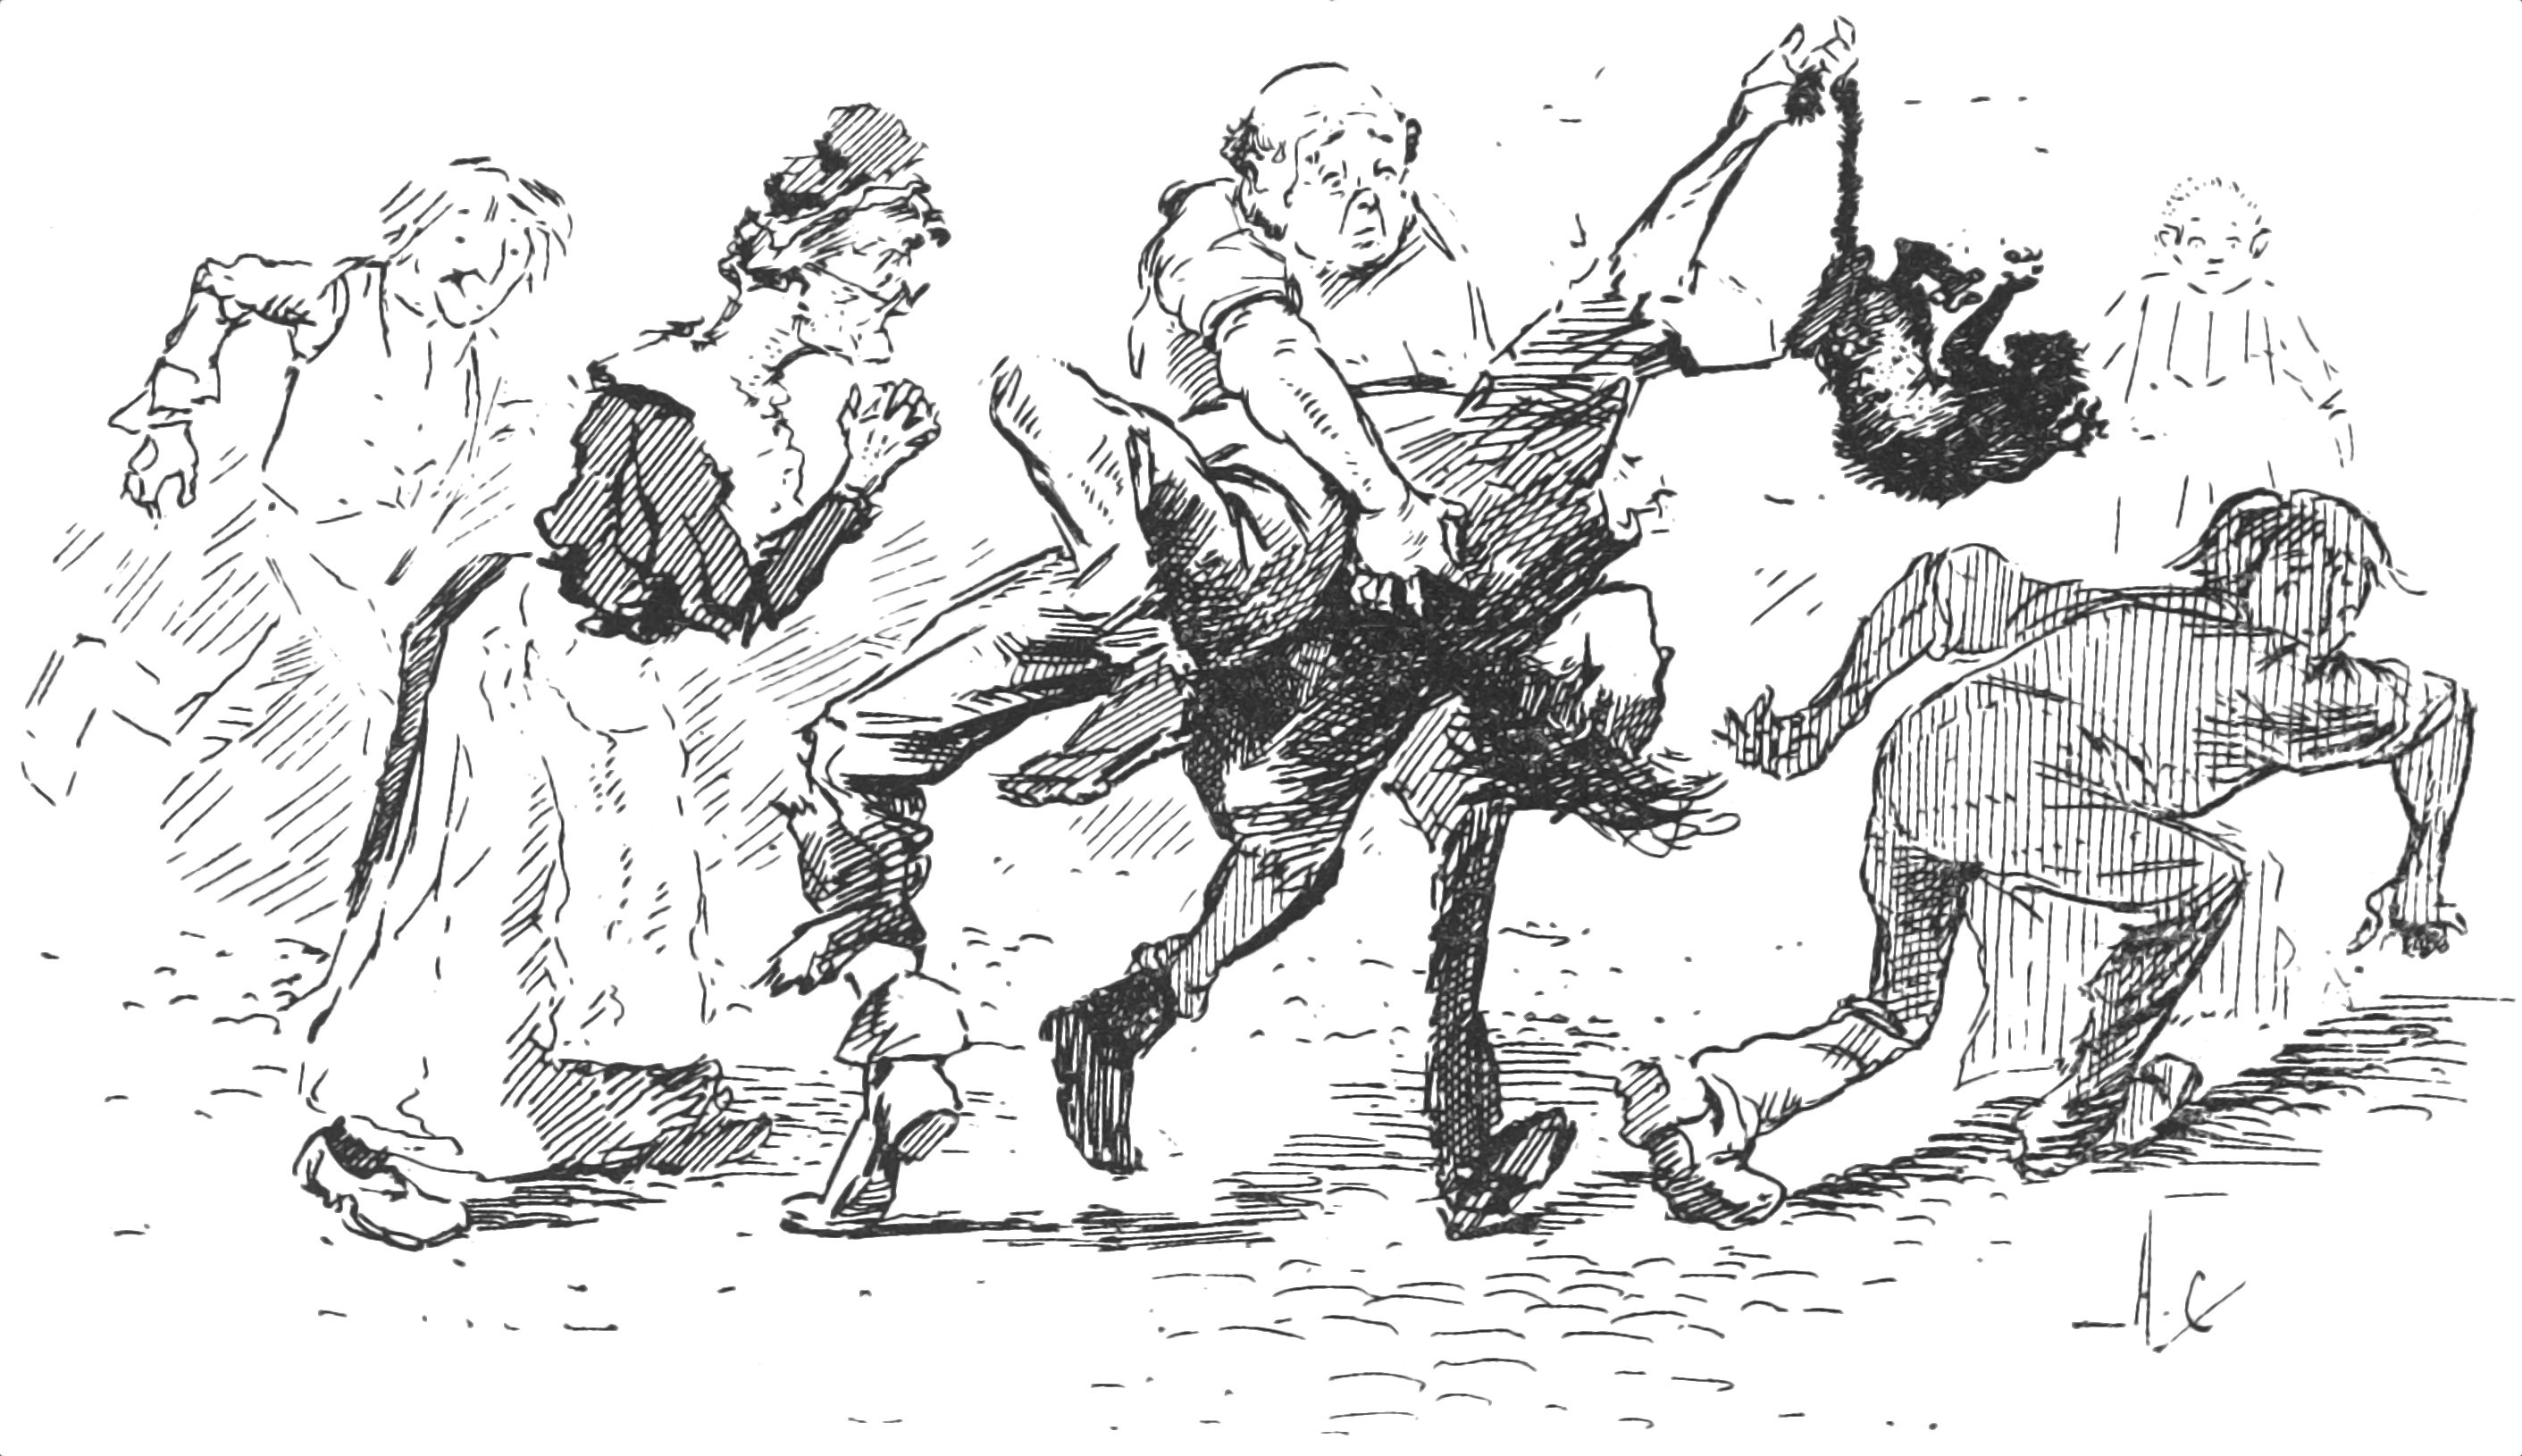
\includegraphics[width=\linewidth]{26parade}
%\caption{Harmless in the brightness of the rising sun}
\end{figure}



All down the line from there the aspect of the country was gaunt and unfamiliar; Wimbledon particularly had suffered. Walton, by virtue of its unburned pine woods, seemed the least hurt of any place along the line. The Wandle, the Mole, every little stream, was a heaped mass of red weed, in appearance between butcher's meat and pickled cabbage. The Surrey pine woods were too dry, however, for the festoons of the red climber. Beyond Wimbledon, within sight of the line, in certain nursery grounds, were the heaped masses of earth about the sixth cylinder. A number of people were standing about it, and some sappers were busy in the midst of it. Over it flaunted a Union Jack, flapping cheerfully in the morning breeze. The nursery grounds were everywhere crimson with the weed, a wide expanse of livid colour cut with purple shadows, and very painful to the eye. One's gaze went with infinite relief from the scorched greys and sullen reds of the foreground to the blue-green softness of the eastward hills.

The line on the London side of Woking station was still undergoing repair, so I descended at Byfleet station and took the road to Maybury, past the place where I and the artilleryman had talked to the hussars, and on by the spot where the Martian had appeared to me in the thunderstorm. Here, moved by curiosity, I turned aside to find, among a tangle of red fronds, the warped and broken dog cart with the whitened bones of the horse scattered and gnawed. For a time I stood regarding these vestiges\textellipsis

Then I returned through the pine wood, neck-high with red weed here and there, to find the landlord of the Spotted Dog had already found burial, and so came home past the College Arms. A man standing at an open cottage door greeted me by name as I passed.

I looked at my house with a quick flash of hope that faded immediately. The door had been forced; it was unfast and was opening slowly as I approached.

%\begin{wrapfigure}{O}{0.5\textwidth}
%\centering
%
\includegraphics[width=0.5\textwidth]{26house}
%\end{wrapfigure}

\begin{figure}[tb]
\centering

\includegraphics[width=\linewidth]{26house}
%\caption{Harmless in the brightness of the rising sun}
\end{figure}

It slammed again. The curtains of my study fluttered out of the open window from which I and the artilleryman had watched the dawn. No one had closed it since. The smashed bushes were just as I had left them nearly four weeks ago. I stumbled into the hall, and the house felt empty. The stair carpet was ruffled and discoloured where I had crouched, soaked to the skin from the thunderstorm the night of the catastrophe. Our muddy footsteps I saw still went up the stairs.

I followed them to my study, and found lying on my writing-table still, with the selenite paper weight upon it, the sheet of work I had left on the afternoon of the opening of the cylinder. For a space I stood reading over my abandoned arguments. It was a paper on the probable development of Moral Ideas with the development of the civilising process; and the last sentence was the opening of a prophecy: »In about two hundred years,« I had written, »we may expect\longdash« The sentence ended abruptly. I remembered my inability to fix my mind that morning, scarcely a month gone by, and how I had broken off to get my \textit{Daily Chronicle} from the newsboy. I remembered how I went down to the garden gate as he came along, and how I had listened to his odd story of »Men from Mars.«

\begin{figure}[tbp]
\centering
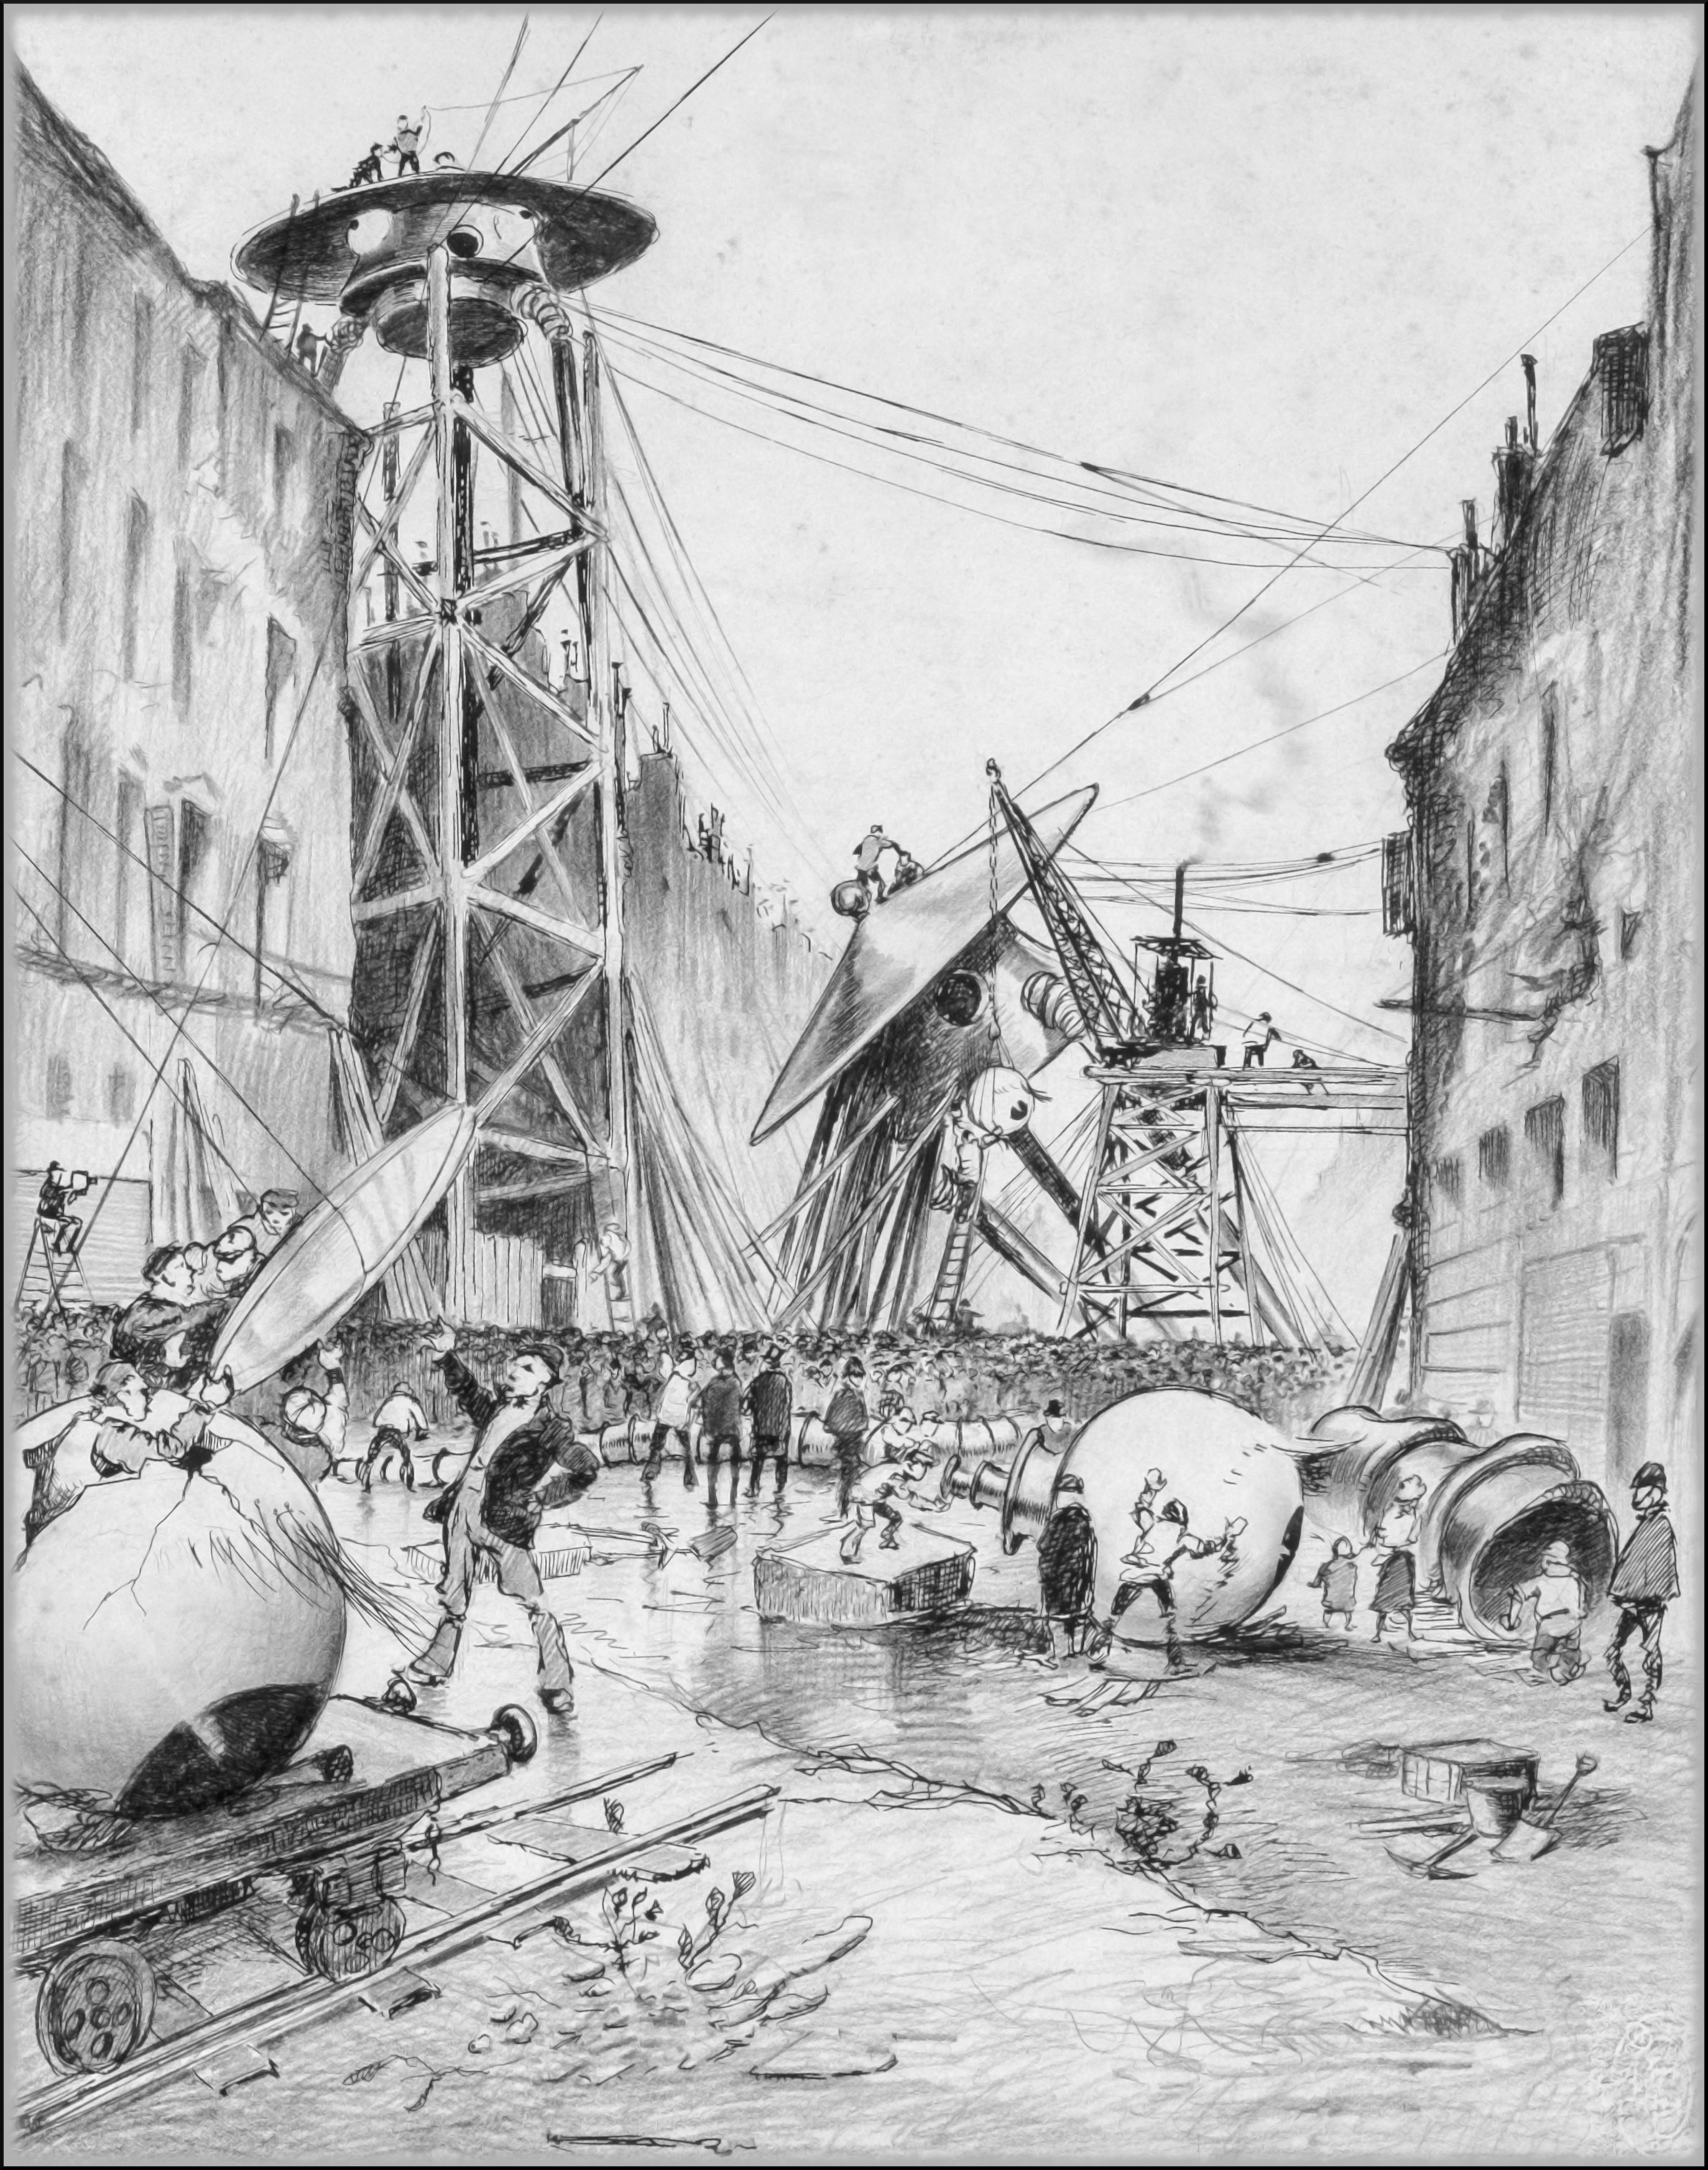
\includegraphics[width=\linewidth]{26astonishing}
\caption[The examination of the Martian mechanisms]{Already in one week the examination of the Martian mechanisms had yielded astonishing results}
\end{figure}

I came down and went into the dining room. There were the mutton and the bread, both far gone now in decay, and a beer bottle overturned, just as I and the artilleryman had left them. My home was desolate. I perceived the folly of the faint hope I had cherished so long. And then a strange thing occurred. »It is no use,« said a voice. »The house is deserted. No one has been here these ten days. Do not stay here to torment yourself. No one escaped but you.«

I was startled. Had I spoken my thought aloud? I turned, and the French window was open behind me. I made a step to it, and stood looking out.

And there, amazed and afraid, even as I stood amazed and afraid, were my cousin and my wife—my wife white and tearless. She gave a faint cry.

»I came,« she said. »I knew—knew\longdash«

She put her hand to her throat—swayed. I made a step forward, and caught her in my arms.

\begin{figure}[b!]
\centering

\includegraphics[width=.5\textwidth]{26tailpiece}
%\captionlistentry{Tailpiece to Chapter \thechapter}
\end{figure}